\section{Pair Testing}
\label{sec:Pair Testing}

Sometimes more than one human beings work together on a single task. If the task is about testing something~\textemdash~welcome to \rindex{\textbf{P}!Pair Testing}Pair testing.

One does the testing and the other analyzes or reviews the testing. They can always switch their roles.

Pair Testing can significantly speed up the testing. One person is a \textbf{Driver}, second is a \textbf{Navigator}. 

\begin{figure}[!h]
\centering
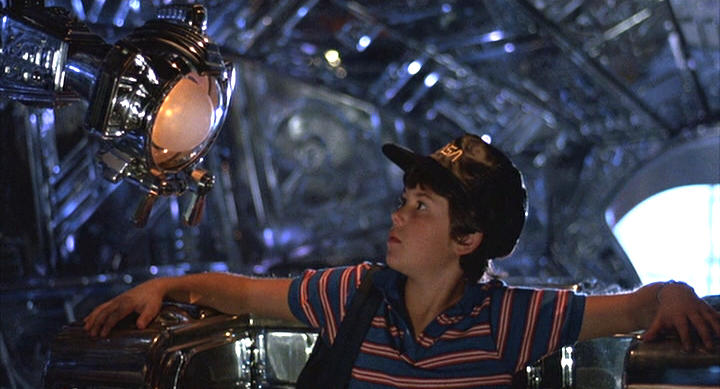
\includegraphics[width=0.8\linewidth]{navigator}
\caption{\ttfamily{Beyond the limits}}
\label{fig:Navigator}
\end{figure}

Both minds can generate testing ideas, and immediately execute them. While Navigator stay for make a note about what was doing and the results, Driver can run and generate next idea, and so on. This can be done between one tester and developer or business analyst or between two testers with both participants taking turns at driving the keyboard. No limits, really!

This approach come from \rindex{\textbf{E}!Exploratory Testing}Exploratory Testing area [p.\pageref{sec:Exploratory Testing}], and it's very controversial. From the manager's point of view, Pair Testing looks like TWO working units do ONE job, so one testing task costs double. While this, will be better if those TWO working units were doing at the same time TWO testing tasks. 

For sure, this if very OK, when the task is to dig a hole at the land. And sometimes testing really looks like digging.

\begin{quote}
You remember the '\textit{You see, in this world there are two kinds of people, my friend: those with a loaded gun and those who dig. You dig}' © from 'The Good The Bad and the Ugly' movie? 

We must understand and admit this truest statement.                                                                                                                                                                                                                                                 \end{quote} 

But there are a lot of tasks in testing, when we need more brains for work, than hands. For such tasks \rindex{\textbf{P}!Pair Testing}Pair Testing can be a wonderful approach, where TWO smart people can work as ONE unit best and quicker than two working units apart.

At the end of Pair Testing this two persons survive so many challenges, that as a nice persons, they have to marry each other, so be careful with this software development technique.
